\documentclass[a4paper]{article}
\usepackage{amsfonts}
\usepackage{amsmath}
\usepackage{amssymb}
\usepackage{graphicx}
\begin{document}

\noindent \large Auteur: Anass Hamzaoui \\
\noindent \large Studierichting: Informatica \\
\noindent \large Oefeningenreeks 5F nr. 2.6 \\
\medskip
\normalsize

$\left|\begin{array}{ll}
    & r_1 = 3: \text{ cirkel, middelpunt } (0,0), \text{ straal } 3 \\
    
    & r_2 = 2\cos\theta: \text{ cirkel, middelpunt } (1,0), \text{ straal } 1 \\
    
    & \max(r_2) = 2 < 3 \implies r_2 \subset r_1 \\
\end{array}\right.$ \\

Grafiek: \\
\begin{figure}[h]
\centering
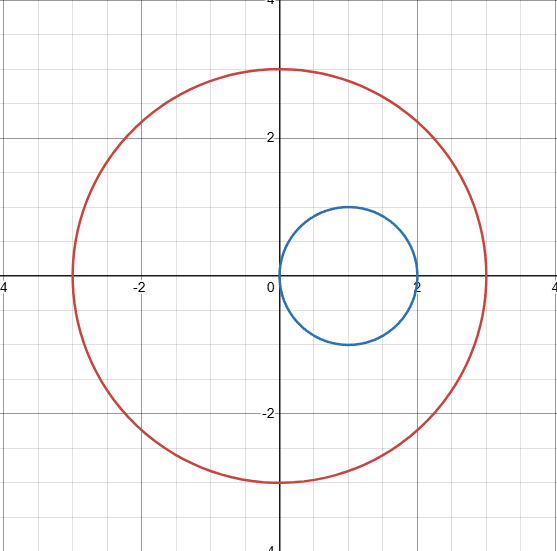
\includegraphics[width=8cm]{5F-2.6-anass.hamzaoui.INF.png}
\end{figure}

$\begin{array}{ll}
S_1 &= \dfrac{1}{2}\displaystyle\int_0^{2\pi} 9  d\theta = \dfrac{9}{2}\left[\theta\right]_0^{2\pi} = 9\pi \\

S_2 &= \dfrac{1}{2}\displaystyle\int_0^{\pi} (2\cos\theta)^2   d\theta = 2\displaystyle\int_0^{\pi} \cos^2\theta   d\theta \\

&= \displaystyle\int_0^{\pi} (1+\cos 2\theta)   d\theta = \left[\theta + \dfrac{\sin 2\theta}{2}\right]_0^{\pi} = \pi \\

S &= S_1 - S_2 = 9\pi - \pi = 8\pi \\
\end{array}$

\begin{thebibliography}{999}
    %\bibitem{a} Referentie
\end{thebibliography}
\end{document}